%%%%%%%%%%%%%%%%%%%%%%%%%%%%%%%%%%%%%%%%%%%%%%%%%%%%%%%%%%%%%%%%%%%%%%
% writeLaTeX Example: A quick guide to LaTeX
%
% Source: Dave Richeson (divisbyzero.com), Dickinson College
% 
% A one-size-fits-all LaTeX cheat sheet. Kept to two pages, so it 
% can be printed (double-sided) on one piece of paper
% 
% Feel free to distribute this example, but please keep the referral
% to divisbyzero.com
% 
%%%%%%%%%%%%%%%%%%%%%%%%%%%%%%%%%%%%%%%%%%%%%%%%%%%%%%%%%%%%%%%%%%%%%%
% How to use writeLaTeX: 
%
% You edit the source code here on the left, and the preview on the
% right shows you the result within a few seconds.
%
% Bookmark this page and share the URL with your co-authors. They can
% edit at the same time!
%
% You can upload figures, bibliographies, custom classes and
% styles using the files menu.
%
% If you're new to LaTeX, the wikibook is a great place to start:
% http://en.wikibooks.org/wiki/LaTeX
%
%%%%%%%%%%%%%%%%%%%%%%%%%%%%%%%%%%%%%%%%%%%%%%%%%%%%%%%%%%%%%%%%%%%%%%

\documentclass[a4paper,10pt,landscape]{article}
\usepackage{graphicx}
\usepackage{multicol,multirow}
\usepackage{calc}
\usepackage{ifthen}
\usepackage[landscape]{geometry}
\usepackage[colorlinks=true,citecolor=blue,linkcolor=blue]{hyperref}
\usepackage{sectsty}
\usepackage{mathtools,amsmath}

\ifthenelse{\lengthtest { \paperwidth = 11in}}
    { \geometry{top=.5in,left=.5in,right=.5in,bottom=.5in} }
	{\ifthenelse{ \lengthtest{ \paperwidth = 297mm}}
		{\geometry{top=1cm,left=1cm,right=1cm,bottom=1cm} }
		{\geometry{top=1cm,left=1cm,right=1cm,bottom=1cm} }
	}

\newenvironment{Figure}
  {\par\medskip\noindent\minipage{\linewidth}}
  {\endminipage\par\medskip}
%\usepackage[landscape]{geometry}
\newcommand{\topic}[1]{\begin{center}\section*{#1}\end{center}}

\begin{document}
\begin{center}
     \Large{\textbf{Cheat-sheet Information Retrieval}} \\
\end{center}
\begin{multicols}{3}
\topic{LSI - Latent Semantic Indexing}
A term document matrix $A_{txd}$ can be decomposed using SVD to:
$A = U\Sigma V^T$
We can see that $\Sigma^{-1}U^TA = V^T$, it therefore seems reasonable to define: $L = U_k\Sigma_k^{-1}$
If lets pretend that $d_i$ is a column of A
Then we can compare documents in the latent space
$sim(d_i,q) = \cos(L^Td_j,L^Tq)$
\topic{pLSA}
Uses 
\begin{Figure}
    \centering
    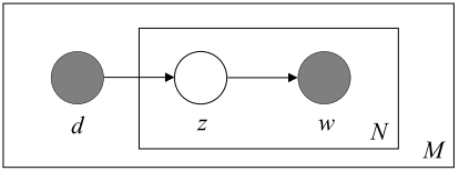
\includegraphics[width=\linewidth]{images/pLSA.png}
    \label{fig:my_label}
\end{Figure}
\begin{Figure}
    \centering
    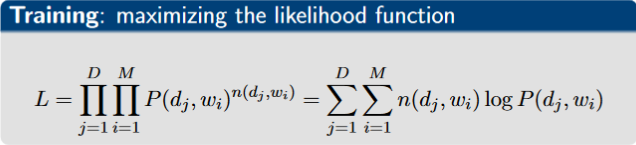
\includegraphics[width=\linewidth]{images/pLSATrain.png}
    \label{fig:my_label}
\end{Figure}
where $n(d_j,w_i) =$ frequency of $w_i\text{ in } d_j$. This is trained with e.g. EM. 
\topic{LDA - Latent Dirichlet Allocation}
\begin{Figure}
    \centering
    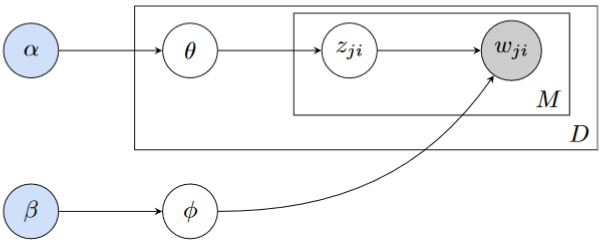
\includegraphics[width=\linewidth]{images/LDA.png}
    \label{fig:my_label}
\end{Figure}

\textbf{Conjugacy of prior:}

Conjugate if $P(X|\theta) \sim A \land P(\theta) \sim B \land P(\theta|X)\sim B$
In our case $z$  is multinomial, therefore the posterior for $\theta$ must be dirichlet (since the prior is also dirichlet).

\textbf{Setting priors}

Good values $\alpha_i = 50/K \beta_i=200/V$

\textbf{Gibbs Sampling}

We fix everything, update the probabilities for z according to:
\begin{equation*}
    P(z_{ji}=k|z_{¬ji},w,\alpha,\beta)\propto \frac{n_{j,k,\negi}+\alpha}{n_{j,k,\negi}+K\alpha}\cdot\frac{v_{k,w_{ji},\neg}+\beta}{v_{k,\neg}+V\beta}
\end{equation*}
Once burned in, sample for each $z_{ji}$. Estimate theta and phi.
\topic{Word Embeddings}
\textbf{CBOW}
Input is words around word to be predicted, trains hidden weight layer.

\textbf{Skip-gram NNLM}
Input current word, predicts surrounding words.
More expensive since need additional weights and softmax.
Basic formulation is:
\begin{equation*}
    p(w_O|w_I) = \frac{exp(v'_{w_O}^Tv_{w_I})}{\sum_{w=1}^{W}exp(v'_{w_O}^Tv_{w_I})}
\end{equation*}
\topic{Feature selection, extraction and learning}
\textbf{$\chi^2$ measure:} Measures the degree of dependence (lack of independence) between an observed probability distribution and an expected distribution.

Definition: $\chi^2(f,c)=\frac{n(n_{++}n_{--}-n_{-+}n_{+-})^2}{n_{c}n_{\sim c}n_{f}n_{\sim f}}$

\textbf{Information Gain}
\textbf{Pointwise mutual information statistic}
\newpage
\end{multicols}

\end{document}